Subbab ini menjelaskan implementasi algoritmik dari sistem navigasi, mencakup \textit{global planner} yang menghasilkan jalur kasar dari awal hingga tujuan, \textit{local planner} berbasis APF yang mengeksekusi penghindaran \textit{obstacle} secara reaktif, mekanisme fusi \textit{traversability} yang mengintegrasikan informasi LiDAR dan termal di dalam APF, serta mekanisme \textit{cat keep-out} yang secara khusus menjaga jarak aman dari \textit{obstacle} rendah yang tidak terdeteksi LiDAR. Keempat komponen ini bekerja secara berlapis dan saling melengkapi pada setiap siklus kendali 10~Hz.

% -----------------------------------------------------------------------
\subsection{Global Planner — \texttt{navfn/NavfnROS}}
\label{sec:global_planner}
% -----------------------------------------------------------------------

\textit{Global planner} bertugas menghasilkan jalur referensi kasar yang menghubungkan posisi robot saat ini dengan titik tujuan. Pada penelitian ini, paket \texttt{navfn/NavfnROS} digunakan sebagai \textit{global planner} yang diintegrasikan ke dalam \texttt{move\_base} melalui antarmuka \texttt{nav\_core::BaseGlobalPlanner}~\cite{Macenski2022}.

Prinsip kerja NavfnROS didasarkan pada algoritma Dijkstra yang dijalankan pada \textit{global costmap} berbasis OGM (\textit{Occupancy Grid Map}). Setiap sel pada grid diberi biaya berdasarkan kedekatannya dengan \textit{obstacle} yang ditandai oleh lapisan \textit{obstacle} (\textit{obstacle layer}). Algoritma Dijkstra kemudian menelusuri sel-sel dari posisi awal hingga tujuan dan memilih rangkaian sel dengan total biaya kumulatif terendah sebagai jalur~\cite{Adiuku2024}. Jalur yang dihasilkan dipublikasikan pada topik \texttt{/move\_base/NavfnROS/plan} dan menjadi referensi bagi APFPlanner.

Pada penelitian ini, \textit{global costmap} mengintegrasikan dua sumber data, yaitu peta statis (\texttt{grit\_1\_edited\_2.yaml}, resolusi 0,05~m/sel) dan lapisan \textit{obstacle} yang mencakup LiDAR (\texttt{/scan}) serta \textit{virtual scan} termal (\texttt{/thermal\_blindspot\_scan}) dengan konfigurasi \texttt{marking=true}. Dengan demikian, posisi \textit{obstacle} kucing yang terdeteksi kamera termal turut dimasukkan ke dalam \textit{costmap} global sebelum NavfnROS merencanakan jalur. Artinya, \textit{global planner} sudah menghasilkan jalur yang secara aktif menghindari area di sekitar kucing, meskipun kucing tidak terlihat oleh LiDAR, sehingga keputusan \textit{routing} tingkat tinggi telah sadar terhadap \textit{blind-spot}~\cite{Fagundes2024}.

Frekuensi \textit{replanning} global ditetapkan pada \texttt{planner\_frequency = 0,2~Hz}, bukan nilai \textit{default} 1,0~Hz. Pilihan ini dilakukan karena \textit{virtual scan} termal bersifat statis dalam jangka pendek: posisi kucing tidak berubah antar-skenario statis, sehingga \textit{replanning} yang terlalu sering justru menimbulkan getaran pada jalur referensi (\textit{path jitter}) yang mengganggu kestabilan APFPlanner. Dengan frekuensi 0,2~Hz, jalur global diperbarui setiap 5~detik, sehingga cukup responsif terhadap perubahan lingkungan tanpa mengganggu kendali lokal.

% -----------------------------------------------------------------------
\subsection{APF \textit{Local Planner}}
\label{sec:apf_planner}
% -----------------------------------------------------------------------

APFPlanner diimplementasikan sebagai \textit{plugin} C++ yang terdaftar ke \texttt{move\_base} melalui antarmuka \texttt{nav\_core::BaseLocalPlanner}. Pada setiap siklus kendali (10~Hz), APFPlanner menerima jalur global dari NavfnROS, membaca data sensor terkini, menghitung gaya total APF, dan menerbitkan perintah kecepatan \texttt{/cmd\_vel} kepada \textit{plugin} kinematik robot~\cite{Khatib1986}.

\subsubsection*{a. Gaya Atraktif}

Gaya atraktif menarik robot menuju \textit{target waypoint} yang dipilih dari jalur global menggunakan strategi \textit{lookahead}: titik pada jalur global yang berjarak $d_\text{look} = 0{,}7$~m dari posisi robot saat ini dijadikan target lokal. Gaya atraktif dihitung sebagai:
\begin{equation}
    \mathbf{F}_\text{att} = k_\text{att}\,\bigl(q_\text{target} - q_\text{robot}\bigr)
    \label{eq:f_att}
\end{equation}
dengan $k_\text{att} = 1{,}5$ sebagai penguatan atraktif (ditetapkan melalui \texttt{nav\_sim.launch}, menggantikan nilai \textit{default} 2,0) dan $q_\text{target} - q_\text{robot}$ sebagai vektor selisih posisi dari robot ke target. Untuk mencegah gaya atraktif yang terlalu besar saat robot masih jauh dari target, besar gaya dibatasi (\textit{clipped}) oleh:
\begin{equation}
    \|\mathbf{F}_\text{att}\| \leq k_\text{att} \cdot d_\text{look}
    \label{eq:f_att_clip}
\end{equation}

\subsubsection*{b. Gaya Repulsif}

Gaya repulsif mendorong robot menjauhi \textit{obstacle} yang terdeteksi dalam radius deteksi \texttt{obs\_detect\_radius} dari data LiDAR \texttt{/scan}. Dari seluruh \textit{obstacle} yang terdeteksi, dipilih \textit{obstacle} terdekat (\textit{closest obstacle}) pada jarak $d_\text{obs}$ dengan posisi $(x_o, y_o)$. Implementasi gaya repulsif mengikuti model Khatib~\cite{Khatib1986}:
\begin{equation}
    F_\text{rep} = G \cdot k_\text{rep} \left(\frac{1}{d_\text{obs}} -
    \frac{1}{d_0}\right) \frac{1}{d_\text{obs}^2}, \quad d_\text{obs} \leq d_0
    \label{eq:f_rep_scalar}
\end{equation}
dengan $k_\text{rep} = 0{,}4$ sebagai penguatan repulsif (dari \texttt{nav\_sim.launch}), $d_0 = 0{,}85$~m sebagai jarak pengaruh \textit{obstacle} pada skenario S1--S3 dan S5--S7 (untuk S4/S8: $d_0 = 1{,}2$~m), serta $G$ sebagai faktor penguatan adaptif yang nilainya bergantung pada konfigurasi. Pada konfigurasi \textit{baseline}, $G = 1{,}0 + (1{,}0 - \tau_\text{trav})$; pada konfigurasi fuzzy, $G = \mathit{rep\_gain}$ yang dihasilkan oleh \textit{fuzzy controller}. Komponen vektor gaya repulsif dalam koordinat dunia adalah:
\begin{equation}
    \mathbf{F}_\text{rep} = F_\text{rep} \cdot
    \frac{q_\text{robot} - q_\text{obs}}{\|q_\text{robot} - q_\text{obs}\|}
    \label{eq:f_rep_vector}
\end{equation}

\subsubsection*{c. Gaya Total dan Kecepatan}

Gaya total yang bekerja pada robot merupakan superposisi gaya atraktif, gaya repulsif, dan gaya \textit{cat keep-out} (yang dibahas pada Subbab~\ref{sec:cat_keep_out}):
\begin{equation}
    \mathbf{F}_\text{total} = \mathbf{F}_\text{att} + \mathbf{F}_\text{rep}
    + \mathbf{F}_\text{cat}
    \label{eq:f_total}
\end{equation}
Vektor $\mathbf{F}_\text{total}$ kemudian ditransformasikan ke koordinat lokal robot dan diskalakan menjadi kecepatan linear $(v_x, v_y)$ yang dibatasi pada $v_\text{max} = 0{,}2$~m/s. Pada konfigurasi fuzzy, kecepatan diskalakan lebih lanjut menggunakan faktor $\mathit{speed\_scale} \in [0, 1]$ dari \textit{fuzzy controller}:
\begin{equation}
    v_x^\text{final} = \mathit{speed\_scale} \cdot v_x, \quad
    v_y^\text{final} = \mathit{speed\_scale} \cdot v_y
    \label{eq:velocity_scale}
\end{equation}
Perlu dicatat bahwa komponen gaya tolak berbasis citra semantik termal (\texttt{thermal\_rep}) dinonaktifkan pada konfigurasi akhir penelitian ini (\texttt{thermal\_rep\_enable = false} di \texttt{nav\_sim.launch}). Penghindaran \textit{obstacle} termal sepenuhnya dilakukan melalui dua jalur yang lebih terstruktur, yaitu \textit{virtual scan} ke \textit{global costmap} untuk menginformasikan perencanaan jalur, serta mekanisme \textit{cat keep-out} berbasis jarak metrik untuk penghindaran lokal \textit{real-time}. Keputusan ini menghindari duplikasi respons tolak yang dapat menyebabkan robot bergerak tidak stabil saat kucing terdeteksi dari dua sumber sekaligus.

\subsubsection*{d. Deteksi Osilasi dan Mode Penghindaran}

Salah satu kelemahan APF klasik adalah osilasi di sekitar \textit{obstacle} pada lorong sempit atau \textit{local minima}~\cite{Lv2024}. APFPlanner mendeteksi osilasi dengan memantau konsistensi arah gaya antar-siklus menggunakan kosinus sudut antara vektor gaya total pada siklus saat ini dan siklus sebelumnya:
\begin{equation}
    \cos\theta_\text{osc} = \frac{\mathbf{F}_\text{total}(t) \cdot
    \mathbf{F}_\text{total}(t-1)}{\|\mathbf{F}_\text{total}(t)\|\,
    \|\mathbf{F}_\text{total}(t-1)\|}
    \label{eq:osc_detect}
\end{equation}
Apabila $\cos\theta_\text{osc} < \theta_\text{thr} = -0{,}5$ (gaya berbalik arah, yang mengindikasikan osilasi), sistem beralih ke mode \textit{AVOIDANCE} selama maksimum 80 siklus ($\approx$8~detik). Dalam mode ini, robot memilih arah manuver berdasarkan zona termal yang lebih lapang (\texttt{zone\_left\_} vs. \texttt{zone\_right\_}), lalu kembali ke mode \textit{NORMAL}.

Tabel~\ref{tab:param_apf} merangkum seluruh parameter APF akhir yang digunakan dalam penelitian.

\begin{table}[H]
\centering
\caption{Parameter akhir APF yang digunakan pada seluruh skenario.}
\label{tab:param_apf}
\begin{tabular}{lllp{5.5cm}}
\toprule
\textbf{Parameter} & \textbf{Notasi} & \textbf{Nilai} & \textbf{Keterangan} \\
\midrule
Penguatan atraktif   & $k_\text{att}$        & 1,5      & Ditetapkan di \texttt{nav\_sim.launch} \\
Penguatan repulsif   & $k_\text{rep}$        & 0,4      & Ditetapkan di \texttt{nav\_sim.launch} \\
Jangkauan pengaruh (S1--S7) & $d_0$         & 0,85~m   & Radius pengaruh gaya tolak \\
Jangkauan pengaruh (S4/S8)  & $d_0$         & 1,20~m   & Diperlebar untuk \textit{obstacle} dinamis \\
Radius deteksi (S1--S7) & $r_\text{det}$     & 0,70~m   & Batas pencarian \textit{obstacle} terdekat \\
Radius deteksi (S4/S8)  & $r_\text{det}$     & 1,30~m   & Diperlebar untuk \textit{obstacle} dinamis \\
Kecepatan linear maks  & $v_\text{max}$      & 0,20~m/s & Batas kecepatan translasi \\
Kecepatan angular maks & $\omega_\text{max}$ & 0,50~rad/s & Batas kecepatan rotasi \\
\textit{Lookahead} distance     & $d_\text{look}$     & 0,70~m   & Jarak target \textit{waypoint} \\
Ambang osilasi         & $\theta_\text{thr}$ & $-0{,}50$ & \textit{Threshold} \textit{cosine similarity} \\
\bottomrule
\end{tabular}
\end{table}

% -----------------------------------------------------------------------
\subsection{\textit{Traversability-Aware}: Fusi LiDAR--Termal}
\label{sec:trav_aware}
% -----------------------------------------------------------------------

Sebagai komponen inti dari kontribusi penelitian ini, APFPlanner dilengkapi dengan fungsi \texttt{computeTraversability()} yang memfusikan informasi geometris dari LiDAR dengan informasi termal dari kamera untuk menghasilkan nilai \textit{traversability} efektif $\tau_\text{eff}$. Nilai ini digunakan secara berbeda pada dua konfigurasi: pada konfigurasi \textit{baseline} (S1--S4), $\tau_\text{eff}$ diwakili oleh \texttt{traversability\_score\_} yang langsung memengaruhi $G$ dalam Persamaan~(\ref{eq:f_rep_scalar}); pada konfigurasi fuzzy (S5--S8), $\tau_\text{eff}$ menjadi salah satu dari dua masukan ke \textit{fuzzy controller}~\cite{Haider2022}.

\subsubsection*{a. Langkah 1 --- Traversability Berbasis LiDAR}

Komponen LiDAR mengukur lebar koridor lateral menggunakan data \texttt{/scan} pada jendela sudut menyamping $[\varphi_\text{lo}, \varphi_\text{hi}] = [0{,}96, 2{,}18]$~rad ($\approx 55^\circ$ hingga $125^\circ$). Jarak lateral ke dinding kiri dan kanan dihitung sebagai:
\begin{equation}
    d_\text{lat} = r_i \cdot \sin|\varphi_i|,
    \quad \varphi_i \in [\varphi_\text{lo},\, \varphi_\text{hi}]
    \label{eq:d_lat}
\end{equation}
Lebar koridor total dan sisa ruang untuk robot diperoleh dari:
\begin{equation}
    w_\text{corridor} = \min_{\varphi_i > 0}\!(d_\text{lat}) +
    \min_{\varphi_i < 0}\!(d_\text{lat}), \quad
    c = w_\text{corridor} - w_\text{robot}
    \label{eq:corridor_m}
\end{equation}
dengan $w_\text{robot} = 0{,}55$~m sebagai lebar fisik robot. Nilai ini dinormalisasi ke rentang $[0, 1]$:
\begin{equation}
    \tau_\text{LiDAR} = \mathrm{clip}\!\left(\frac{c}{\,c_\text{ref}\,},\;0,\;1\right)
    \label{eq:trav_lidar_apf}
\end{equation}
dengan $c_\text{ref} = 0{,}25$~m sebagai nilai clearance yang dianggap sebagai kondisi "koridor penuh" ($\tau = 1{,}0$). Nilai $c_\text{ref}$ yang relatif kecil ini ditetapkan agar $\tau_\text{LiDAR}$ mencapai 1,0 bahkan pada koridor yang tidak terlalu lebar, sehingga faktor pembatas $\tau$ yang lebih dominan adalah komponen termal.

\subsubsection*{b. Langkah 2 --- Koreksi Termal dengan Low-Pass Asimetris}

Nilai \textit{traversability score} dari kamera termal ($\tau_\text{thermal}$ dari topik \texttt{/traversability\_score}) difilter menggunakan \textit{low-pass filter} eksponensial dengan konstanta $\alpha$ yang berbeda bergantung pada arah perubahan (Persamaan~(\ref{eq:lpf_alpha}) dan~(\ref{eq:lpf_update}) pada Subbab~\ref{sec:fusi_trav}). Penggunaan $\alpha_\text{turun} = 0{,}50$ yang lebih besar daripada $\alpha_\text{naik} = 0{,}20$ berarti sistem bereaksi dua kali lebih cepat saat \textit{obstacle} panas muncul dibandingkan saat \textit{obstacle} pergi. Ini merupakan pilihan desain yang disengaja untuk memprioritaskan keamanan.

\subsubsection*{c. Langkah 3 --- Fusi dengan Operator Minimum}

Nilai $\tau_\text{eff}$ diperoleh sebagai nilai minimum antara kedua komponen, sesuai dengan Persamaan~(\ref{eq:trav_eff}):
\begin{equation}
    \tau_\text{eff} = \min\!\bigl(\tau_\text{LiDAR},\; \hat{\tau}_\text{thermal}\bigr)
    \label{eq:trav_eff_repeat}
\end{equation}
Operator minimum dipilih berdasarkan prinsip konservatif: sistem merespons sumber bahaya mana pun yang memberikan sinyal lebih negatif, baik dari koridor LiDAR yang sempit maupun dari area termal yang terhalang \textit{obstacle} panas~\cite{Schichler2025}. Gambar~\ref{fig:traversability_fusi} mengilustrasikan alur fusi ini.

\begin{figure}[H]
    \centering
    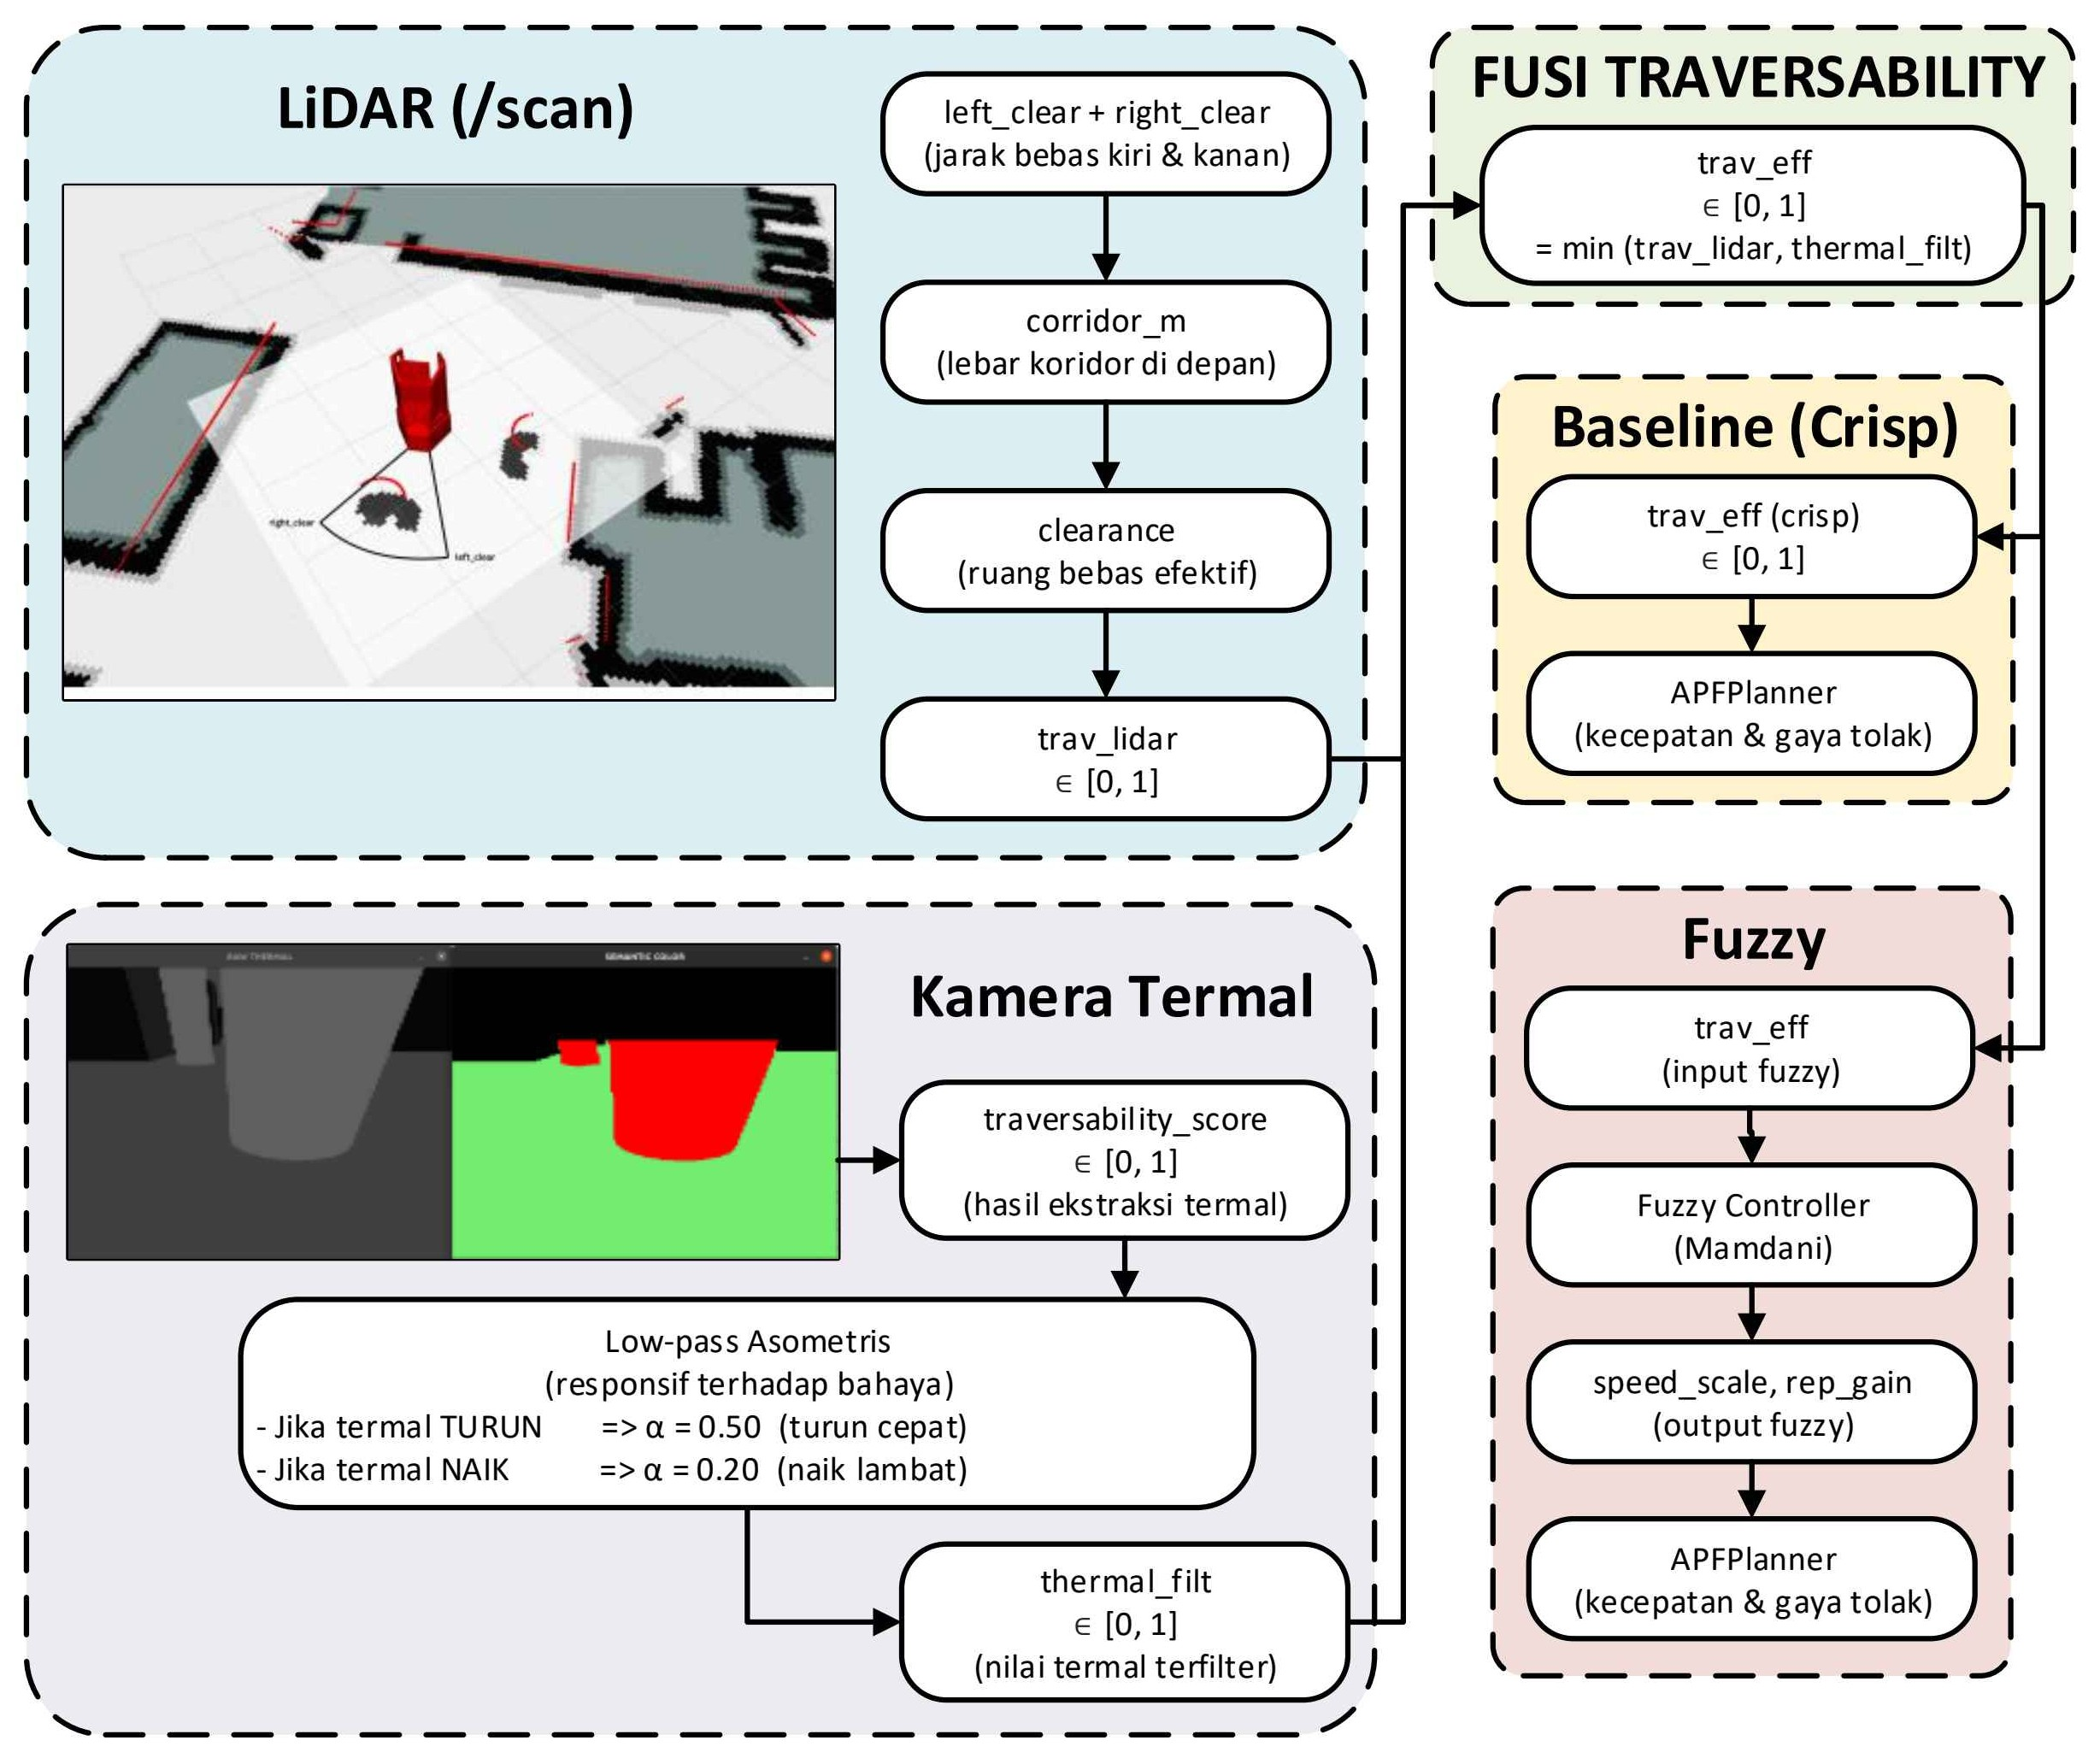
\includegraphics[width=0.75\textwidth]{gambar/3.6_traversability_fusi.jpg}
    \caption{Diagram alur fusi \textit{traversability} LiDAR--termal pada fungsi \texttt{computeTraversability()}. Jalur LiDAR (atas): jarak bebas kiri dan kanan dari pindaian \texttt{/scan} pada jendela sudut samping menghasilkan $\tau_\text{LiDAR} \in [0,1]$. Jalur termal (bawah): \textit{traversability score} dari kamera termal difilter oleh LPF asimetris ($\alpha=0{,}50$ saat turun, $\alpha=0{,}20$ saat naik) menghasilkan $\hat{\tau}_\text{thermal}$. Keduanya difusikan dengan operator minimum menghasilkan $\tau_\text{eff}$, yang kemudian digunakan sebagai masukan \textit{fuzzy controller} (S5--S8) atau langsung memengaruhi penguatan repulsi \textit{crisp} (S1--S4). \textit{Inset} kiri bawah menunjukkan contoh tampilan segmentasi termal saat kucing (\textit{merah}) terdeteksi di depan robot.}
    \label{fig:traversability_fusi}
\end{figure}

% -----------------------------------------------------------------------
\subsection{\textit{Cat Keep-Out} dan \textit{Latch} Berbasis Jarak}
\label{sec:cat_keep_out}
% -----------------------------------------------------------------------

Mekanisme \textit{cat keep-out} adalah komponen yang secara khusus menangani \textit{obstacle} rendah yang tidak terdeteksi LiDAR (yaitu kucing), dengan memanfaatkan informasi metrik dari \textit{virtual scan} termal \texttt{/thermal\_blindspot\_scan}. Mekanisme ini hanya aktif pada konfigurasi fuzzy (\texttt{use\_fuzzy = true}, skenario S5--S8) dan berfungsi sebagai lapisan keamanan tambahan di luar mekanisme gaya repulsif APF konvensional.

\subsubsection*{a. Penguncian Posisi Kucing (\textit{Latch})}

Saat \textit{virtual scan} termal mendeteksi objek panas pada jarak $r_\text{blind}$ dan sudut $\varphi_\text{blind}$ (beam dengan nilai finite pada \texttt{/thermal\_blindspot\_scan}), APFPlanner mengunci estimasi posisi kucing dalam \textit{frame} dunia:
\begin{equation}
    \begin{bmatrix} x_\text{cat} \\ y_\text{cat} \end{bmatrix} =
    \begin{bmatrix} x_\text{robot} \\ y_\text{robot} \end{bmatrix} +
    (r_\text{blind} + r_\text{cat}) \cdot
    \begin{bmatrix} \cos(\psi + \varphi_\text{blind}) \\
                    \sin(\psi + \varphi_\text{blind}) \end{bmatrix}
    \label{eq:cat_world}
\end{equation}
dengan $\psi$ sebagai orientasi robot, dan $r_\text{cat} = 0{,}18$~m sebagai radius kucing. Penambahan $r_\text{cat}$ memindahkan estimasi dari permukaan ke pusat kucing.

Setelah posisi dikunci, sistem menerapkan \textit{latch} berbasis jarak: posisi yang dikunci dipertahankan dan gaya \textit{keep-out} terus aktif selama jarak robot ke kucing masih berada di dalam zona pengaruh $d_{0c}$, tanpa memperhatikan apakah kucing saat ini terlihat atau tidak oleh kamera. Kunci baru dilepaskan hanya apabila robot telah jelas melewati kucing, yaitu saat jarak ke kucing melampaui $d_{0c} + 0{,}5$~m dan tidak ada deteksi baru selama $> 1{,}0$~detik. Desain \textit{latch} ini memastikan bahwa satu deteksi termal yang singkat sudah cukup untuk menjaga margin sepanjang proses melintas, meskipun kucing keluar dari FOV kamera saat robot menyusur di sebelahnya.

\subsubsection*{b. Jarak Aman (\textit{Safe Distance})}

Pusat robot dijaga agar selalu berjarak minimal $D_\text{safe}$ dari pusat kucing:
\begin{equation}
    D_\text{safe} = r_\text{cat} + \frac{w_\text{robot}}{2} + \delta_\text{margin}
    \label{eq:d_safe}
\end{equation}
dengan $r_\text{cat} = 0{,}18$~m, $w_\text{robot}/2 = 0{,}275$~m (setengah lebar robot), dan $\delta_\text{margin} = 0{,}08$~m sebagai batas aman tambahan. Dengan demikian, $D_\text{safe} = 0{,}18 + 0{,}275 + 0{,}08 = 0{,}535$~m. Zona pengaruh \textit{keep-out} meluas hingga $d_{0c} = D_\text{safe} + \delta_\text{infl}$, dengan $\delta_\text{infl} = 0{,}18$~m (\texttt{cat\_influence = 0,18}, ditetapkan di \texttt{nav\_sim.launch}), sehingga $d_{0c} = 0{,}715$~m.

\subsubsection*{c. Gaya \textit{Keep-Out}}

Gaya radial yang mendorong robot menjauhi kucing dihitung sebagai berikut. Misalkan $d_\text{cat} = \|q_\text{robot} - q_\text{cat}\|$ adalah jarak pusat robot ke pusat kucing, dan $\delta_d = d_\text{cat} - D_\text{safe}$ adalah selisih terhadap batas aman ($\delta_d > 0$: robot di luar batas, $\delta_d < 0$: robot melanggar batas). Besar gaya \textit{keep-out} dihitung menggunakan fungsi \textit{ramp} kuadratik:
\begin{equation}
    f_\text{cat} =
    \begin{cases}
        G_\text{cat} \cdot t^2, & \delta_d > 0,\ t = \dfrac{d_{0c} - d_\text{cat}}{\delta_\text{infl}} \\[6pt]
        G_\text{cat} \cdot \bigl(1 + 12\,|\delta_d|\bigr), & \delta_d \leq 0 \quad \text{(pelanggaran)}
    \end{cases}
    \label{eq:f_cat_scalar}
\end{equation}
dengan $G_\text{cat} = 3{,}0$ sebagai penguatan \textit{keep-out} (\texttt{cat\_keep\_gain}). Saat robot masih berada di luar $D_\text{safe}$ tetapi di dalam $d_{0c}$, gaya berbentuk kuadratik (naik halus dari nol menuju $G_\text{cat}$ saat mendekati batas). Saat robot telah melampaui $D_\text{safe}$ ($\delta_d \leq 0$), gaya melonjak tajam dengan faktor linier tambahan untuk mendorong robot keluar segera. Arah gaya selalu radial menjauhi posisi kucing:
\begin{equation}
    \mathbf{F}_\text{cat} = f_\text{cat} \cdot
    \frac{q_\text{robot} - q_\text{cat}}{\|q_\text{robot} - q_\text{cat}\|}
    \label{eq:f_cat_vector}
\end{equation}

Kontribusi $\mathbf{F}_\text{cat}$ terhadap $\mathbf{F}_\text{total}$ (Persamaan~(\ref{eq:f_total})) bekerja secara sinergis dengan gaya atraktif yang terus menarik robot ke arah tujuan. Gabungan keduanya menghasilkan trajektori yang secara natural menyusur melewati sisi kucing yang searah dengan tujuan, tanpa memerlukan perencanaan trajektori eksplisit. Tabel~\ref{tab:param_cat} merangkum seluruh parameter mekanisme ini.

\begin{table}[H]
\centering
\caption{Parameter \textit{cat keep-out} yang digunakan pada konfigurasi fuzzy (S5--S8).}
\label{tab:param_cat}
\begin{tabular}{llll}
\toprule
\textbf{Parameter} & \textbf{Notasi} & \textbf{Nilai} & \textbf{Keterangan} \\
\midrule
Radius kucing       & $r_\text{cat}$          & 0,18~m & Dari dimensi model Gazebo \\
Setengah lebar robot & $w_\text{robot}/2$     & 0,275~m & Dari \textit{footprint} kotak \\
Margin aman         & $\delta_\text{margin}$  & 0,08~m & Ruang bebas tepi-ke-tepi \\
Jarak aman pusat    & $D_\text{safe}$         & 0,535~m & Dari Persamaan~(\ref{eq:d_safe}) \\
Zona pengaruh       & $\delta_\text{infl}$    & 0,18~m & \texttt{cat\_influence}, dari \texttt{launch} \\
Batas zona pengaruh & $d_{0c}$                & 0,715~m & $D_\text{safe} + \delta_\text{infl}$ \\
Penguatan \textit{keep-out} & $G_\text{cat}$  & 3,0    & \texttt{cat\_keep\_gain} \\
Waktu \textit{latch} & $t_\text{latch}$       & 1,0~det & Batas waktu tanpa deteksi baru \\
Batas jarak lepas kunci & $d_{0c} + 0{,}5$ & 1,215~m & Robot dianggap sudah lewat \\
\bottomrule
\end{tabular}
\end{table}